\documentclass[12pt,a4paper,utf8x]{report}
\usepackage [frenchb]{babel}

% Pour pouvoir utiliser 
\usepackage{ucs}
\usepackage[utf8x]{inputenc}

\usepackage{url} % Pour avoir de belles url
\usepackage {geometry}

% Pour mettre du code source
\usepackage {listings}
% Pour pouvoir passer en paysage
\usepackage{lscape}

% Pour pouvoir faire plusieurs colonnes
\usepackage {multicol}
% Pour crééer un index
\usepackage{makeidx}
\makeindex

% Pour gérer les liens interractifs et les signets Acrobat
\usepackage{hyperref}
\hypersetup{
pdftitle={titre de mon document},
pdfauthor={Nom de l'auteur},
pdfsubject={Sujet du document},
pdfkeywords={les mots clefs},
bookmarks, % Création du signet
pdfstartview=FitH, % Page de la largeur de la fenêtre
colorlinks=true, % Liens en couleur
linkcolor=black, 	
anchorcolor=black, 	
citecolor=black, 	
filecolor=black, 	
menucolor=black,
runcolor=black,
urlcolor=black, 	
frenchlinks=black,
bookmarksnumbered=true, % Signet numéroté
pdfpagemode=UseOutlines, % Montre les bookmarks.
bookmarksopen =true,
}

% Pour afficher la bibliographie, mais pas nottoc (Table of Contents), notlof (List of Figures) ni notlot (List of Tables)
\usepackage[notlof, notlot]{tocbibind}


% Pour les entetes de page
% \usepackage{fancyheadings}
%\pagestyle{fancy}
%\renewcommand{\sectionmark}[1]{\markboth{#1}{}} 
%\renewcommand{\subsectionmark}[1]{\markright{#1}} 

% Pour l'interligne de 1.5
\usepackage {setspace}
% Pour les marges de la page
\geometry{a4paper, top=2.5cm, bottom=3.5cm, left=1.5cm, right=1.5cm, marginparwidth=1.2cm}

\parskip=5pt %% distance entre § (paragraphe)
\sloppy %% respecter toujours la marge de droite 

% Pour les pénalités :
\interfootnotelinepenalty=150 %note de bas de page
\widowpenalty=150 %% veuves et orphelines
\clubpenalty=150 

%Pour la longueur de l'indentation des paragraphes
\setlength{\parindent}{15mm}



%%%% debut macro pour enlever le nom chapitre %%%%
\makeatletter
\def\@makechapterhead#1{%
  \vspace*{50\p@}%
  {\parindent \z@ \raggedright \normalfont
    \interlinepenalty\@M
    \ifnum \c@secnumdepth >\m@ne
        \Huge\bfseries \thechapter\quad
    \fi
    \Huge \bfseries #1\par\nobreak
    \vskip 40\p@
  }}

\def\@makeschapterhead#1{%
  \vspace*{50\p@}%
  {\parindent \z@ \raggedright
    \normalfont
    \interlinepenalty\@M
    \Huge \bfseries  #1\par\nobreak
    \vskip 40\p@
  }}
\makeatother
%%%% fin macro %%%%

%Couverture 

\title
{
	\normalsize{
	University of Nantes\\
	2009-2010}\\
	\vspace{15mm}
	\Huge{AtariGo technical report}
}
\author{CAILLAUD Anthony \and FORTUN Manoël \\
	\vspace{45mm}
}


\begin{document}

\maketitle

\tableofcontents
\clearpage

% Pour avoir un interligne de 1,5
\begin{onehalfspace}

\chapter{Introduction}

This report explain some technical feature of our AtariGo project. We will see some explanation about the use of our software. How the game works. How to improve this software. We will present some class diagram about the architecture. Some specific algorithm will be detailled.



\clearpage


\chapter{Model View Controler}

For our project as it were composed by a graphical user interface (UI), we have choose to implement a kind of model view controler pattern as seen in the figure \ref{mvc}.

  \begin{figure}[h!]
  \centering

  \scalebox{1}{
        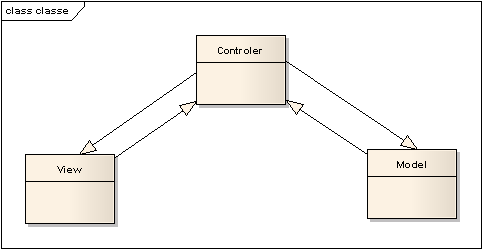
\includegraphics{image/MVCmodel}
  }

  \caption{Our MVC}
\label{mvc} 
 \end{figure}

As you will see on the diagram we not respect entirely the pattern. In the classical way of this pattern, the view is notified automatically if there is any change in the model, and the view directly ask the model of the change. In our way if the model change, the model tell the controler that tell the view, and the view ask the controler for the change.

All the transaction pass threw the controler, the controler is the kind of the master of the application it really make the links between the others perspective. 

All the action on the UI are transfert by actionListener to the controler that transfert to the model.

Our view is compose by the "fr.alma.ihm" package, this package containt all the graphical component for the UI.

Our controler is composed by the "fr.alma.controler" package, this package containt the controler, that "know" all the other perspective, and this package containt a factory, this factory is used to construct the different action listener.

Our model is composed by the "fr.alma.model" package, this package containt all the rule to play, the representation of the board and the class that is the AI.

Now we will see details about the different package and algorithm.


\clearpage


\chapter{The view}

The diagram on figure \ref{view} represent the actual package of the view. We see different class of the UI. All those class containt different graphical element, and represent different aspect of the UI.

  \begin{figure}[h!]
  \centering
  \scalebox{0.7}{
      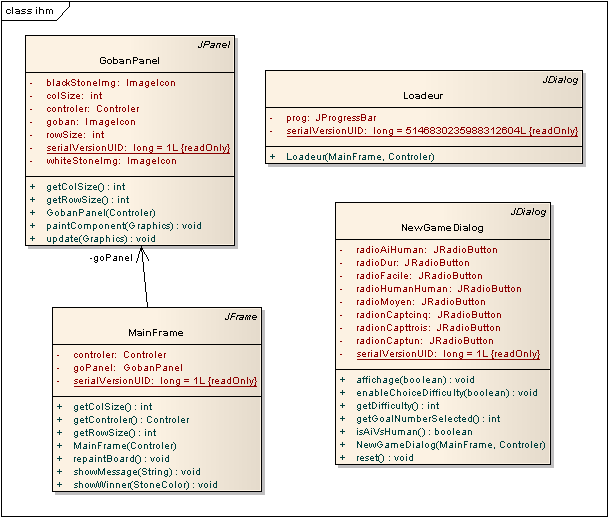
\includegraphics{image/ihm_class_diagram}
  }
  \caption{the view package}
\label{view} 
 \end{figure}



\clearpage


\chapter{The controler}


The diagram on figure \ref{controler} represent the actual package of the controler.  As we can see the controler is all mighy, is "knows" the view and the model. The ActionListenerFactory just construct action listener for the different action, all the action are transfered to the controler that dispatch after. The controler does not do anything else than transfert action and reaction, it does not calcul anything. 


  \begin{figure}[h!]
  \centering
  \scalebox{0.7}{
      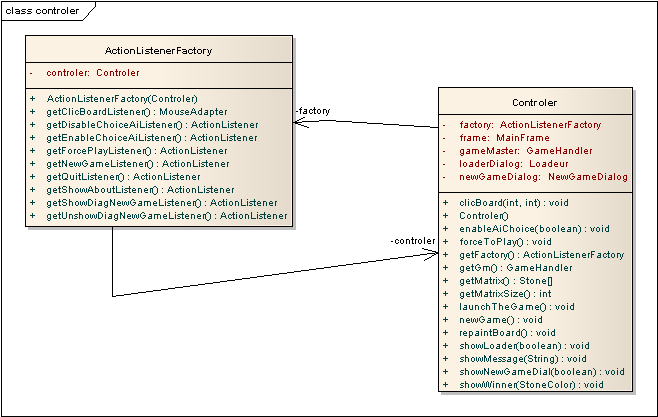
\includegraphics{image/controler_class_diagram.png}
  }
  \caption{the controler package}
\label{controler} 
 \end{figure}



\clearpage


\chapter{The model}

\subsection{Base package}

The diagram on figure \ref{model1} represent the first part of the package. In this diagram we can see the base of the game, there are the stone, the group that represent group of stone, coordinate of the stone and the color. All classes are the base of the game. 

The class group containt simple management of the collection it own and a special feature to melt group together. The method works simply, it take the groupe the bigger and transfert all the stone in this group and it add the liberty of the smallest group in the bigest, and set the group of all the stone to the biggest, and it return the final group.

  \begin{figure}[h!]
  \centering
  \scalebox{0.5}{
      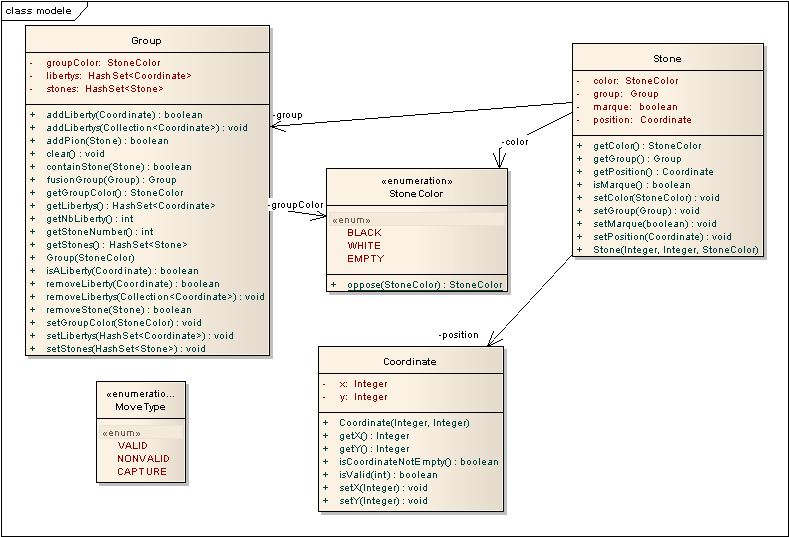
\includegraphics{image/model_class_diagram_part1.png}
  }
  \caption{Model package part1}
\label{model1} 
 \end{figure}

The diagram on figure \ref{model2} represent the second part of the package. In this diagram we can see the "heart" of the game, it containt the actual board and all the method to add stone, it manage the game's rules. All this process is manage by the goban class. 

The Gamehandler is kind of the model manager, it manage the AI, the board, if the ai is activate and a move play by the player, the gamehandler will tell to the AI to play. It check if there is a winner.

The goban class is the board and all the method relative to the game evolution. It containt method to add stone, to remove stone, to handle capture, to check if a move is allowed, etc. 

To check if a move is allowed, it check if there not a stone already on the slot, it check if there is liberty for the stone, but if there no liberty for the stone but remove the last liberty of an enemy group, the move is allowed.

The goban class offer other utility method like get the liberty list of a stone, the neighbors of a stone.

This class handle two mode of game evolution, one that remove stone on the board if there a capture and a one that don't remove stone, the second one is used by the AI to prepare move and see if it capture stone. This last mode is use with the removeStone method that reform the group(by backtraking the stone formation's), it works better is the game is not corrupted by the AI move.

  \begin{figure}[h!]
  \centering
  \scalebox{0.5}{
      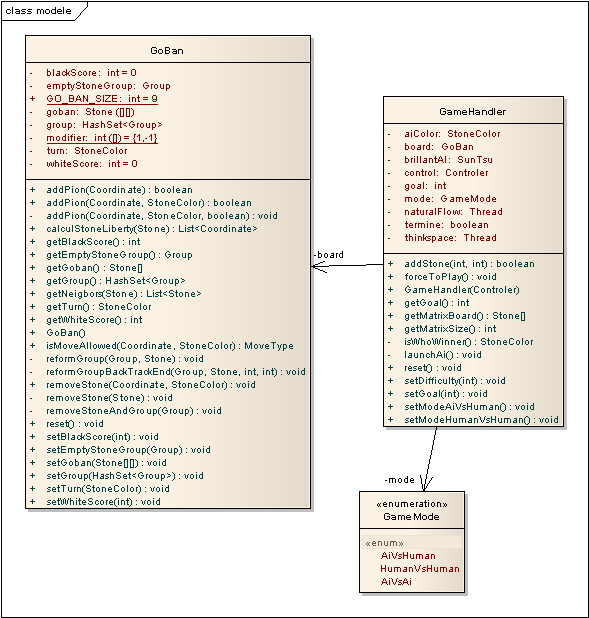
\includegraphics{image/model_class_diagram_part2.png}
  }
  \caption{Model package part2}
\label{model2} 
 \end{figure}


\subsection{Intelligence package}

The diagram on figure \ref{intel} represent the sub package inteligence. In this diagram we can see the "brain" of the game, our brillant(or not) AI with a awesome name. This package contain all the class used by the AI to calculate the "best" move. 

The algorithm to calculate the best move is basically the AlphaBeta algorithm, but every intermediary result is store for the case of an interruption of the calculation. 

To have the possibility of interrupt the calculation, the calculation is launch in a new thread by the gameHandler class, and after another thread wait for the result, it use the wait() method, then when the calculation is over, the thread who wait the result is notify() that is not have to wait more time. To interrupt the calculation it just have to notify() and then the result thread will get an intermediary result.


  \begin{figure}[h!]
  \centering
  \scalebox{0.6}{
      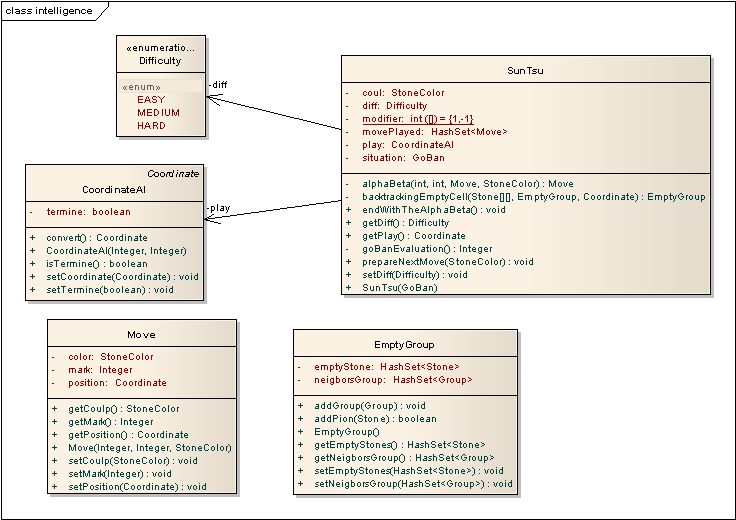
\includegraphics{image/model_intelligence_class_diagram.png}
  }
  \caption{Intelligence sub package}
\label{intel} 
 \end{figure}

The evaluation of a situation is made by the SunTsu class, it check the liberty of all groups, it check if there some eyes in the game by backtracking groups of empty cells, if there so surround by one group it is an eye.


\clearpage


\chapter{Conclusion}

If you want to add some feature don't forget our MVC pattern and it's use. The AI can, has, to be improve by change how it calculate the mark of a situation, actually it's not the better solution that were coded. Diagram are aviable in the image folder so detail will be more visible.

% Pour finir l'interligne de 1,5
\end{onehalfspace}

%----------------------------------------
% Pour la bibliographie
%----------------------------------------
% Citer tous les ouvrages/références
\nocite{*}
% Trier par ordre d'apparition
\bibliographystyle{unsrt}
% Pour le style de la biblio
\bibliographystyle{plain.bst}
% Ecrire la biblio ici
\bibliography{biblio}

\printindex

\appendix


\end{document}
